\section{HLS based BFS optimization} \label{sec:bfs-opt}
BFS is a system.
We need optimize the whole system from pre-processing to hardware pipelining.
This work centers the FPGA acceleration but it also needs assitance of a coupled CPU 
which can either be connected via PCIE or a shared memory structure.
We works on CSR data. irregular memory access? random memory accesses -->low bandwidth.
 memory access conflict, it is difficult to resolve the conflict using HLS. 
Try to explore on-chip memory bandwidth. We use bitmap to store the vivsiting status.
A single FPGA nowadays can already accommodate Graphs with millions of nodes.
pipelined BFS structure.

\begin{itemize}
\item pre-processing, graph reordering and padding
\item on-chip buffering and parallel data path II = 2
\item batch write
\item CPU assisted data reorganization
\end{itemize}

presents the overview of 
the BFS accelerator. It targets in-memory graphs on a PCIe based 
high performance FPGA card. The whole graph is stored in FPGA device 
memory with a standard CSR format. 
Ideally, the accelerator does the BFS on FPGA without 
any interference from the host CPU. However, we organize the accelerator 
following the data flow model of Xilinx HLS and the data flow model 
doesn't allow feedback from the downstream stages to previous stages.
(Detailed BFS data flow will be illustrated in the next section.)
As a result, we can only put one BFS iteration on FPGA while 
leaving the iterative execution control to the host CPU. In each BFS iteration, 
the BFS kernel on FPGA returns the BFS frontier size to host such that the host will 
decide if another BFS iteration should be invoked. Although short communication 
between the host and FPGA in each BFS iteration is needed, the communication cost 
is negligible compared to the execution time. Hereby, 
the overall BFS runtime is barely affected.

The BFS algorithm is critical to the BFS accelerator and we explore the 
existing level synchronous BFS algorithm in detail. We notice that 
the level synchronous BFS algorithm may have redundant vertices pushed to the 
frontier queue in a parallel architecture especially when the frontier grows larger.
The main reason roots in the large amount of overlapped neighbor vertices among the 
frontier vertices as mentioned in previous section. When the frontier neighbors 
are inspected in parallel for faster BFS traverse, these overlapped vertices may be 
considered as frontiers independently and inserted into the next frontier queue. 
As a result, there may be redundant vertices put into the frontier queue and it is 
rather complex to get rid of the redundancy \textit{completely}. Although the redundant 
vertices in the frontier will not cause any BFS mistakes, they will soon lead to large 
amount of redundant traverses recursively and degrade the BFS performance.

To address this problem, we analyze the frontier from the 
vertex status in each BFS iteration to completely cut down the 
propagation of the redundant frontier vertices as proposed in prior 
GPU based BFS acceleration \cite{liu2015enterprise}. The modified algorithm is described 
in Algorithm \ref{alg:modified-bfs}. Instead of inspecting on the frontier vertices directly, 
it starts with vertex status analysis and inspects the frontier 
in each BFS iteration. Although it seems the additional frontier inspection stage 
brings more memory access, the inspection processing are complete sequential 
memory access and can be done efficiently. It is still worth for the overhead 
when compared to the cost caused by the redundant frontier vertices. 
The rest part of the algorithm from line 10 to 15 is 
quite similar to the level synchronous BFS except that the frontier queues 
are no longer needed.


With the observations in Section \ref{sec:observation} 
and the modified BFS algorithm in Section \ref{sec:overview}, 
we start to optimize the BFS accelerator using high level design tools 
from a series of different angles. First of all, we convert the nested loop structure 
of the BFS to be a stream manner such that it can be fit into the data flow model in
Xilinx HLS for efficient pipelined execution. Then we explore a series of memory optimization 
techniques based on the BFS memory access characteristics observed in \ref{sec:observation}. 
Afterwards, we further apply some general HLS optimizations to the resulting design. Finally, 
we manually tune the design parameters such as the prefetch buffer size and cache size through 
the fast software emulation and provide optimized configurations for each graph data set.

\subsection{BFS pipelining}
The baseline BFS algorithm is a multi-level nested loop with 
dynamic memory accesses. It is quite challenging for the HLS 
tools to produce optimized hardware by adding the HLS pragmas to 
the native high level code directly because of the following two 
reasons. First of all, inner most loop and outer loop body can't be pipelined 
automatically by the HLS tools unless the inner most loop is fully 
unrolled and pipelined. Nevertheless, the inner most loop in BFS 
can't be fully unrolled because of the dynamic loop structure.  
Secondly, the outer loop nests access memory randomly even though 
these accesses are actually sequential because they must wait 
for the execution of the inner loop nest which can't 
be fully pipelined. This will lead to low 
memory bandwidth utilization. Similar problem also happens when the 
loop body is complex and different parts of the loop body fail to be 
pipelined properly. In summary, applying HLS pragmas to the native high level BFS code 
will produce low efficient design and the performance of the resulting hardware 
can be far from satisfying.  

To address these problems, we divide the BFS algorithm into pipelined 
sub functions. Basically, there are generally two rules that 
we can create pipelined functions. 
First of all, each loop nest can be packaged into a sub function 
and the dependent sub functions can be pipelined. There are four loop 
nests in Algorithm \ref{alg:modified-bfs}, 
but the loop in line 12 actually include two loops as we need to go through 
both the CSR row and column to obtain a frontier neighbor's index. Thus we 
actually have five sub functions following this rule. Secondly, complex loop body 
can be split to more fine-grained sub functions such that the dependent parts can 
be executed in parallel with additional buffers between them. 
In BFS inner most loop, we can further divide the \textit{depth} read and write 
operations to two dependent sub functions. We can 
do more partitions and create even deeper pipelines, while there is no 
guarantee for always better performance and more hardware resources 
are usually required.

Following the two pipelining rules, we create a six-stage 
pipelined BFS algorithm as detailed in Algorithm \ref{alg:bfs-stream}. 
The six sub functions are labeled as f1 to f6 respectively. In f1, 
vertex status is read from FPGA DDR memory sequentially through a streaming port. 
When the vertex status is fetched, f2 inspects the status 
flowed from the stream buffer, decides the current frontier 
and dumps the frontier to the downstream pipeline. 
With the frontier stream, f3 can further fetch graph 
data stored as CSR. CSR includes a row pointer array (RPA) 
and a column index array (CIA), and they must be sequentially accessed. 
In f3, we combine each pair of RPA entry of the frontier as a construct 
and pass it to the next stream function f4. When f4 gets the RPA pair, 
it can read the CIA sequentially through a streaming port. 
When data in CIA stream which is essentially the potential 
next frontier vertices are received in f5, their vertex status 
will be checked by reading the vertex status array stored in DDR as well.
Only the vertices that are not visited yet will be further forwarded to the f6. 
In f6, the vertex status will be updated.

\begin{algorithm}
	\caption{Pipelined BFS Algorithm} \label{alg:bfs-stream}
    \small
	\begin{algorithmic}[1]
        \Procedure {BFS}{}
        \State $frontier\_size \gets 1$
        \State $level \gets 0$
        \While {$(frontier\_size > 0)$}
        \State $f1(depth, depth\_stream)$
        \State $f2(depth\_stream, frontier\_stream, level, frontier\_size)$ 
        \State $f3(frontier\_stream, CSR.RPA, RPA\_stream)$
        \State $f4(RPA\_stream, CSR.CIA, CIA\_stream)$ 
        \State $f5(CIA\_stream, depth, next\_frontier\_stream)$
        \State $f6(depth, next\_frontier\_stream, level)$
        \State $level \gets level + 1$
        \EndWhile
        \EndProcedure
        \State

        \Procedure{f1}{$depth$, $depth\_stream$}
        \For {$v \in V$}
        \State $depth\_stream << depth[v]$
        \EndFor
        \EndProcedure

        \Procedure{f2}{$depth\_stream, frontier\_stream, level, frontier\_size$}
        \State $frontier\_size = 0$
        \For {$v \in V$}
        \State $d[v] \gets depth\_stream.read()$
        \If {$(d[v] == level)$}
        \State $frontier\_stream << v$
        \State $frontier\_size++$
        \EndIf
        \EndFor
        \EndProcedure

        \Procedure{f3}{$frontier\_stream, CSR.RPA, RPA\_stream$}
        \While {$(!frontier\_stream.empty())$}
        \State $v \gets frontier\_stream.read()$
        \State $RPA\_stream << [CSR.RPA[v], CSR.RPA[v+1]]$
        \EndWhile
        \EndProcedure

        \Procedure{f4}{$RPA\_stream, CSR.CIA, CIA\_stream$}
        \While {$(!RPA\_stream.empty())$}
        \State $[begin, end] \gets RPA\_stream.read()$
        \For {${v \in CSR.CIA(begin, end)}$}
        \State $CIA\_stream << v$
        \EndFor
        \EndWhile
        \EndProcedure

        \Procedure{f5}{$CIA\_stream, depth, next\_frontier\_stream$}
        \While {$(!CIA\_stream.empty())$}
        \State $v \gets CIA\_stream.read()$
        \If {$(depth[v] == -1)$}
        \State $next\_frontier\_stream << v$
        \EndIf
        \EndWhile
        \EndProcedure

        \Procedure{f6}{$depth, next\_frontier\_stream, level$}
        \While {$(!next\_frontier\_stream.empty())$}
        \State $v \gets next\_frontier\_stream.read()$
        \State $depth[v] \gets level + 1$
        \EndWhile
        \EndProcedure

    \end{algorithmic}
\end{algorithm}

According to the description of the streamed BFS algorithm, we notice that 
five sub functions involve external memory access and they have quite different 
memory access patterns. The memory access patterns are summarized in 
Figure \ref{fig:bfs-stream}. f3 reads all the vertex status and 
it has a long sequential memory read. f2 reads the CSR row pointer of the frontier, 
and it reads two sequential words each time. f1 reads the CSR column index and the 
burst length depends on the vertex degree which varies in a large range. 
f4 and f5 involves vertex status reads and writes of the next frontier vertices.
As these vertices are not sequential, the HLS tools just take them as random access 
without any specific hints from the designers. 

\begin{figure}
\center{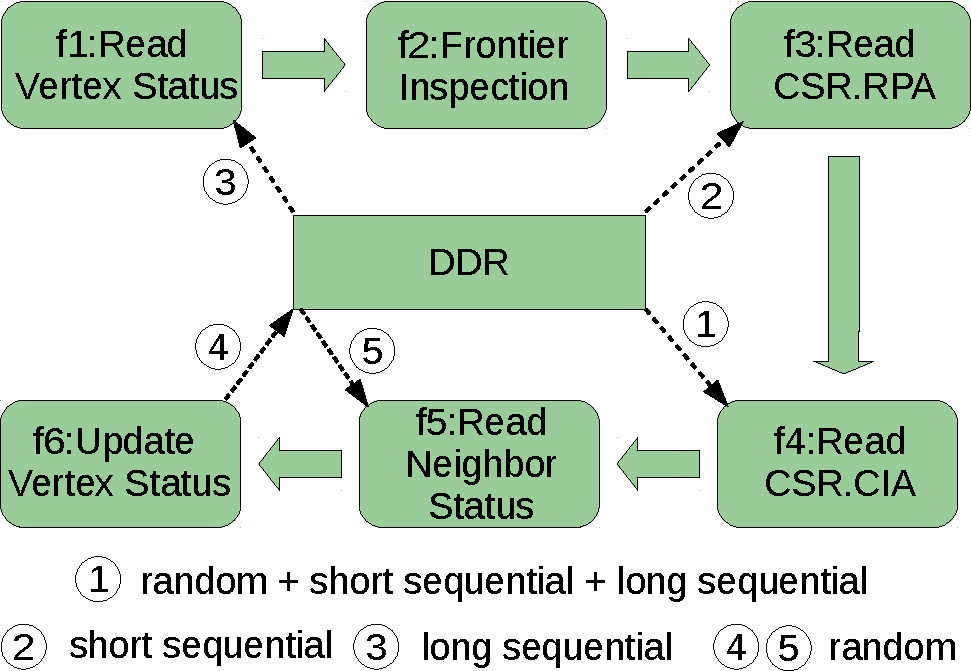
\includegraphics[width=0.65\linewidth]{bfs-stream}}
\caption{Streamed BFS Algorithm}
\label{fig:bfs-stream}
\end{figure}

\subsection{Memory Access Optimization}
As observed in Section \ref{sec:observation}, memory access especially the random and 
short sequential memory accesses are critical to the 
BFS performance. In this sub section, we will mainly explore the memory 
access optimization techniques based on the observations on top of 
the pipelined BFS design.

\subsubsection{Redundancy Removal}
There are many redundant vertices among the frontier neighbors in BFS. 
They may further cause unnecessary vertex status reads and writes in 
f5 and f6 respectively. In order to remove the redundant memory access 
and improve the memory bandwidth utilization, we create hash tables 
to perform the redundancy removal. As the redundant vertices are 
relatively random, a big hash table can be utilized to squeeze 
the redundancy. However, big hash table degrades the hardware implementation 
frequency and eventually lowers the overall performance. Hereby, we 
build a series of smaller hash tables and apply them in parallel. 
The hash table based redundancy removal structure is shown in Figure \ref{fig:hash-strategy}. 
We use the lower bits of the data address as the hash function 
for the sake of better timing. An input data that fails to find a 
record in any of the hash tables will be considered to be a unique 
data and put into one of the hash tables to avoid repeated data 
going through the filter. In order to ensure balanced hash 
table utilization, we implement a hardware-friendly round robin 
arbiter to decide the hash table updating order. 
  
\begin{figure}
\center{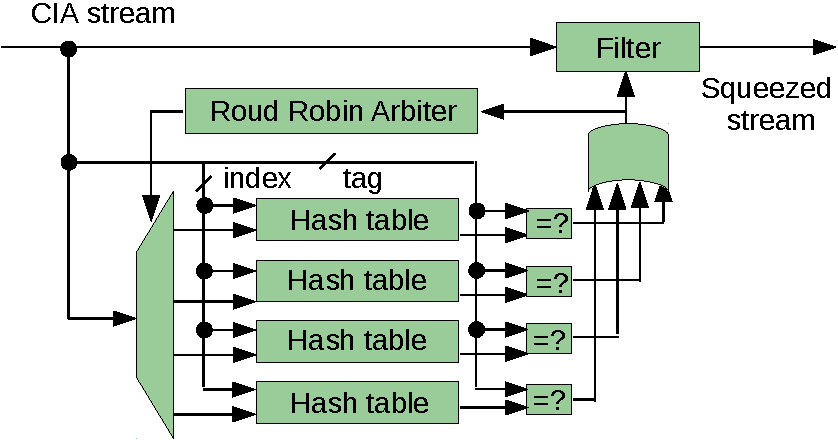
\includegraphics[width=0.75\linewidth]{hash-strategy}}
    \caption{Redundancy removal based on parallel hash tables.}
\label{fig:hash-strategy}
\end{figure}

\subsubsection{Caching}
According to the experiments in Section \ref{sec:observation}, 
there are many random memory accesses and short 
sequential memory accesses in f5 and f6. 
It is generally difficult to optimize these memory accesses. Fortunately, 
the spatial locality analysis shown in the observation experiments 
implies the great potential of cache based memory access optimization. 
Inspired by the observation, we developed an HLS based cache specifically 
for the vertex status \textit{depth} access. 

Since the cache is only used for \textit{depth} array read and write, we  
choose the \textit{depth} array index instead of its physical address for cache 
indexing. Each cache line is set to be 512-bit which is equal to the recommended 
memory access data width and a single memory read or write operation can 
fulfill the requirement of the cache operations including cache read miss, 
cache write miss and cache write back. Since the cache can't be shared 
between different SDAccel data flow functions, a natural cache design is 
to implement both cache in f5 and f6. Both cache can be relatively simple 
for supporting only read operations in f5 and write operations in f6.  

In this work, we choose the directly mapped cache for the BFS optimization. 
Cache line size is set to be 64B which fits well with the optimized global memory 
access port data width.
Although set associative cache architectures will achieve higher 
cache hit rate, the benefit is mostly compromised by the degraded 
implementation frequency on Alpha Data FPGA board. The trade-off 
may be different on a more advanced FPGA boards, but the optimization 
philosophy is pretty much similar. 
 
\subsubsection{Prefetching}
According to the BFS algorithm, the frontier is sequentially inspected. 
Therefore, the CSR information is also accessed in one direction 
in f3 and f4, though they are not necessarily sequential. Basically 
both the column array index and the row column index will increase 
monotonically in one BFS iteration. The CSR data will not be repeatedly 
referenced through the BFS. To optimize these memory 
accesses, a small prefetch buffer 
is build to improve the memory access efficiency. 

Prefetch buffer is also an important design parameter that needs to be tuned.
The general design trade-off is complex.
A larger prefetch buffer improves the hit rate, but it may incur more memory 
access cost and waste the memory bandwidth if the prefetched data are 
not fully used. Meanwhile, larger prefetch buffer adds prefetching cost 
when there is prefetch buffer miss, which may degrade the performance. 
A smaller prefetch buffer typically lead to lower hit rate though 
the prefetched data will be mostly used. Nevertheless, we notice that 
prefetching data that is smaller than 64B will not have clear advantages on timing 
nor memory bandwidth utilization compared to 64B prefetch buffer. 
On the other hand, prefetching more than 64B data doesn't have 
significant hit rate improvement and even results in 
performance drop mainly due to the increase of the prefetch cost when there 
is prefetch buffer miss. In this case, 64B is set to be the prefetch buffer size 
in the end.

\subsection{General HLS optimization}
On top of the pipelining, redundancy removal and caching, there are also 
many other relatively general design optimizations that can improve the 
resulting BFS accelerator performance. These optimizations will be briefly 
introduced in this sub section.

\subsubsection{Data path duplication}
When the DDR memory bandwidth is not saturated, a simple 
yet efficient optimization method is to duplicate the data paths. 
With multiple parallel BFS data paths, the accelerator can issue more parallel 
memory requests pushing higher memory bandwidth utilization. A straightforward 
way of data path duplication is to split the vertex status into different 
partitions and each partition is processed by an instance of the same BFS data path.

However, this method may not work as good as expected for three reasons. 
First of all, the vertices in the frontier may not distribute evenly across the graph. 
As a result, the different pipelines may have unbalanced workloads. Secondly, 
when the cache is applied to the pipelined data path, the same cache line may 
have multiple copies stored in f6 cache and this may cause 
cache coherence problem when they are modified differently 
and written back to memory independently. Finally, duplicating 
the non-bottleneck pipeline stages will not be beneficial to 
the final performance while it incurs more hardware resource consumption 
including not only the basic FPGA cells but also the global memory ports. 

To address the problems, we propose a delicate data path duplication strategy 
as shown in Figure \ref{fig:duplicate-pipeline}. According to the BFS algorithm, 
we know that each frontier vertex requires two CSR row pointer read and multiple 
CSR column index read. Thus the bottleneck pipeline stages may probably start 
from f3. In this case, we split the stream generated in f3 into 
multiple streams. Each sub stream will be handled independently by a 
duplicated data path. This also solves the data path load balancing problem 
naturally. Finally, to ensure a simple yet efficient cache coherence, we 
merge the output stream of f5 into a single stream before flowing into the 
last f6 stage with a write cache. 

\begin{figure}
\center{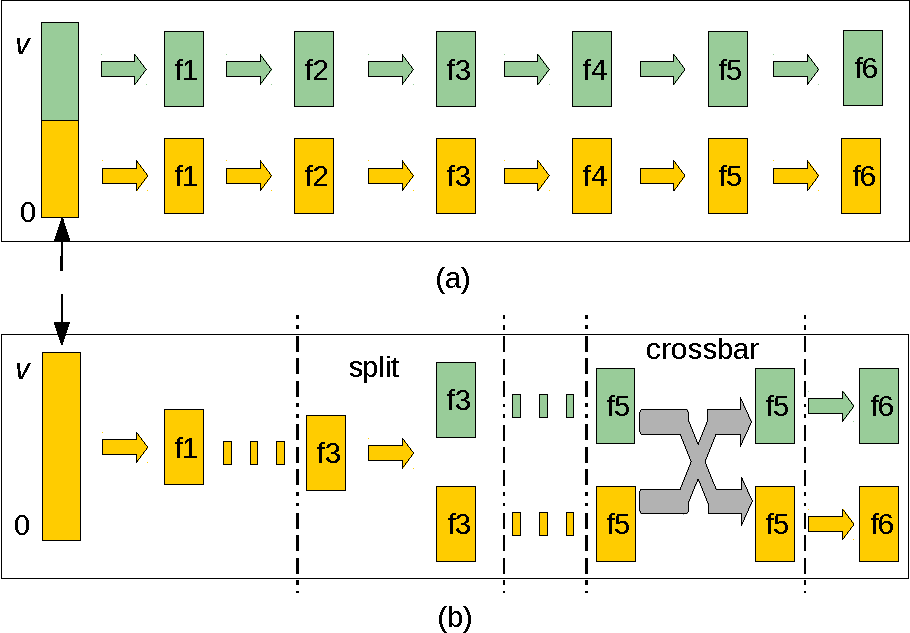
\includegraphics[width=0.85\linewidth]{pipeline-duplication}}
    \caption{pipeline duplication. (a) straightforward pipeline duplication 
    (b) optimized pipeline duplication.}
\label{fig:duplicate-pipeline}
\end{figure}


\subsubsection{Data width optimization}
The memory bandwidth utilization is sensitive to the data width setup. 
According to our experience, sequential memory access 
with 512-bit data width achieves the optimal memory bandwidth. With this guideline, 
a lot of design parameters such as the cache line size and prefetch length are 
set to be 512-bit for higher memory bandwidth utilization. For sequential 
memory access with smaller data width such as 32-bit, we must ensure that the 
data is aligned to 512-bit through padding the access. Otherwise, writing 
unaligned data may corrupt the data in memory.

%\subsubsection{II optimization}
%In the pipelined design, initialization interval (II) indicates the 
%processing throughput. Larger II in a single pipeline stage 
%may slow down the rest of the system. Thus we try to reduce II of all 
%the pipelined sub functions. In particular, hash table, cache and prefetch 
%buffer may affect the II. Inappropriate implementation may lead to 
%large II and even compensate the benefits brought by these optimizations. 

\subsubsection{Deadlock removal}
Another challenge of the pipelined BFS accelerator design is the 
unexpected deadlock problem. 
When a pipeline stage issues a long burst request to the memory 
but gets stalled due to the insufficient read buffer, it has to 
wait for the downstream pipeline stages to consume the data in the buffer. 
However, the downstream pipeline stages may also be stalled due to 
the failure of acquiring the bus that is taken by the upstream pipeline stage.
It is difficult to debug and resolve this deadlock. To address this problem, we
add additional user buffer in the pipeline stages with long sequential 
memory access and split the long sequential memory access into smaller 
segments such that each segment can be accommodated by the buffer. 
Although this may cause slightly lower bandwidth utilization, it breaks the deadlock and 
ensures the correctness of the pipelined design.

\subsection{Parameter Tuning}
As presented in previous sub sections, there are quite some design 
parameters such as hash table size and cache design, 
that need to be explored. However, exploring the design parameters 
based on the hardware implementation directly requires many lengthy 
hardware implementations (A typical BFS implementation may 
take 1 hour to 4 hours to complete.) which is extremely time-consuming.

In this work, we manually tune the design paramters. To obtain the optimized 
design parameters rapidly, we extract a series of hardware implementation independent 
metrics such as cache hit rate and hash table hit rate 
through faster software emulation mode in SDAccel which typically completes in a few minutes.
With these metrics, we can roughly decide the prefetch buffer size, 
cache size and hash table size etc. Afterwards, we go through the lengthy 
hardware implementation and choose the best parameters based on the final 
run time. A more systematic design parameter tuning will be helpful, but it 
is beyond the scope of this work and we will leave it for our future work.

%\subsection{Parameter tuning}
%In this work, we manually tune the design parameters. To obtain the 
%optimized design parameters rapidly, we proposed a general HLS design 
%parameter tuning flow for the HLS based design. The design flow is 
%presented in Figure \ref{fig:parameter-tuning}. It includes three 
%iterative loops tuning different types of the design parameters.
%
%The first loop replies on the fast software emulation which is 
%immediately available using HLS.
%With the software emulation, we can extract a set of statistical 
%metrics such as cache hit rate, prefetch hit rate that are 
%mostly independent with the hardware implementation. These metrics can be used to 
%guide the cache and prefetch buffer design. Although they 
%are not sufficient to decide the exact accelerator performance, they 
%can help prune the design options that are far from optimal and thus reduce 
%the design parameter tuning time. The second tuning loop is based on the hardware 
%pre-synthesis which is also fast and can be done in a few minutes. 
%With the pre-synthesis report, we can optimize the II by 
%improving the HLS design. When the potential design 
%configurations gets smaller, we can get into the last loop and start the time consuming 
%hardware implementation evaluating the configurations with the real 
%performance or resource metrics. Finally, we would like to emphasize the verification process, 
%it needs to be enabled all the time, as optimization may also cause mistakes of the resulting design.
%
%\begin{figure}
%\center{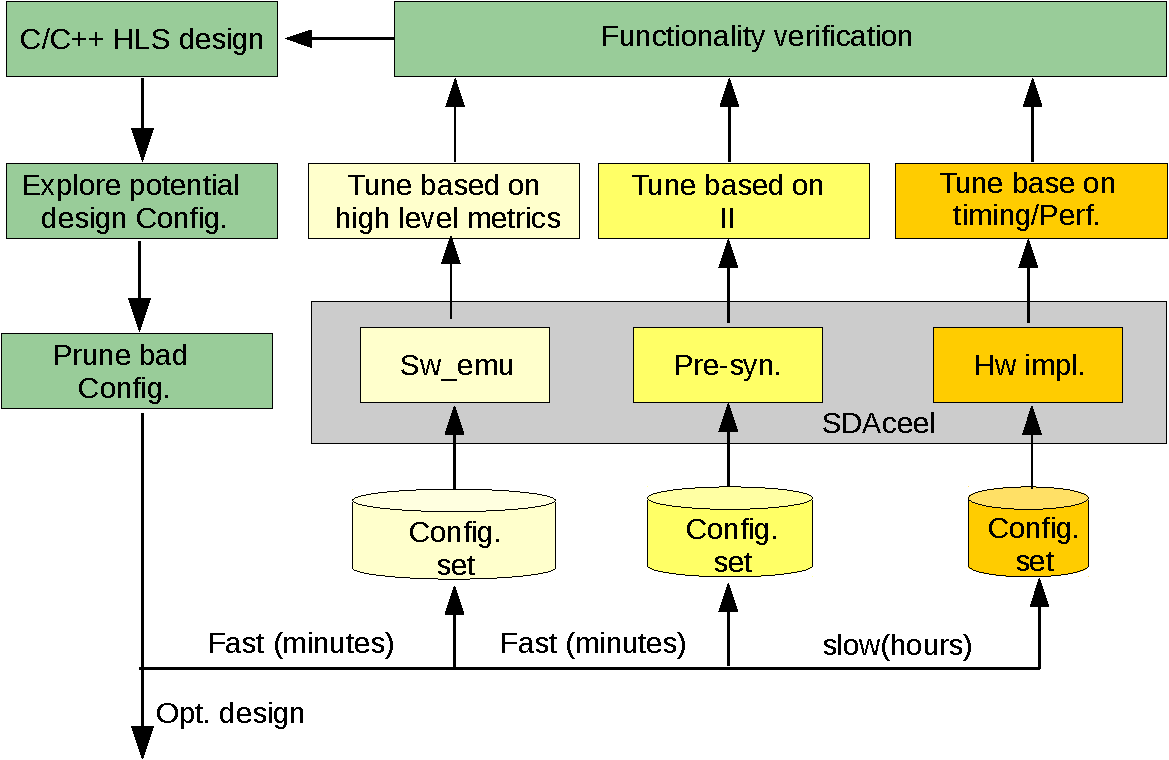
\includegraphics[width=0.95\linewidth]{parameter-tuning}}
%    \caption{Design parameter tuning flow based on SDAccel.}
%\label{fig:parameter-tuning}
%\end{figure}
%

%\appendix
%\section{Acknowledgement}

%\begin{acks}
%  The authors would like to thank Sam Ho for providing the suggestions on
%  HLS design debugging and optimization as well as the SDAccel usage. 

%\end{acks}
